% !TEX root = ../../seminar.tex

\subsection {Scientific Method}
\label{subsec:scientific method}

mapping of our process to scientific method\\
our states mapped to the states given in the graph of scientific method using color of our workflow graph. no additional inserts done.\\
the mapping shows, that we have more fine grained resolotion in the parts around experimenting. this foccus is motivated by the students as target group.
since a advisor usually gives students a research question,our graph lacks the part with observations and thinking of questions and maps 3 states and two transitions to just the two yellow ones of the \checklist.
We do not fully agree with refining, altering or expanding the hyptothesis based on experiment results. From our point of view, these findings should be reported and put in larger context like other findings and evoke a new supgraph with the new arising questions.


\begin{figure}
	\centering
	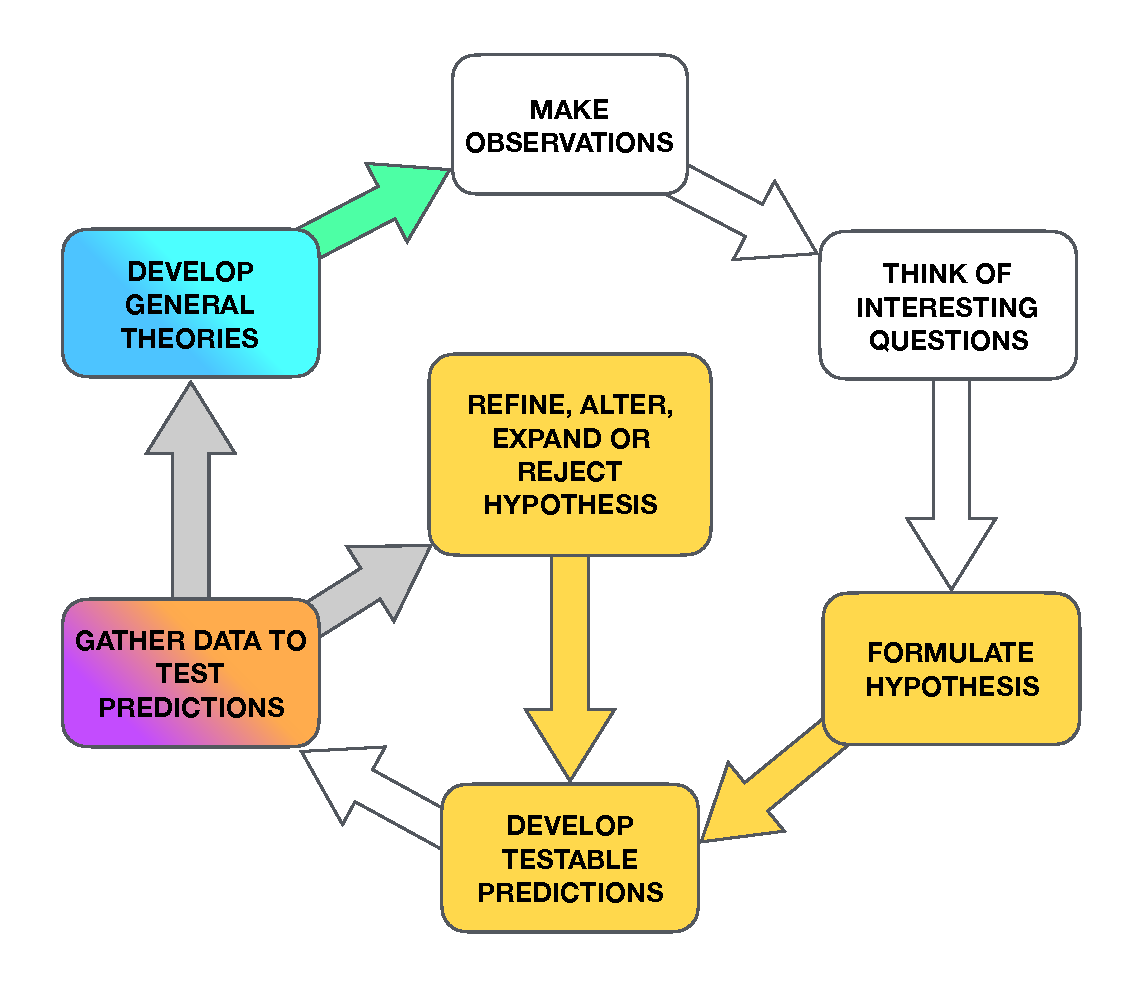
\includegraphics[width=12cm]{figures/scientific_method_mapping.pdf}
	\caption{Mapping of our process to the scientific method. \todo{source for graph}}
	\label{fig:PICOT_FINER}
\end{figure}


